%%%%%%%%%%%%%%%%%%%%%%%%%%%%%%%%%%%%%%%%%%%%%%%%%%%%%%%%%%%%%%%%%%%%%%%%
%Desarrollo de un juego para Nintendo DS | Trabajo de Fin de Grado
% Escuela Politécnica Superior de la Universidad de Alicante
% Realizado por: Carla Maciá Díez
% Contacto: carlamd1997@hotmail.com / cmd23@alu.ua.es
%%%%%%%%%%%%%%%%%%%%%%%%%%%%%%%%%%%%%%%%%%%%%%%%%%%%%%%%%%%%%%%%%%%%%%%%

\chapter{Conclusiones}

En este apartado vamos a repasar el estado actual del proyecto, las posibles mejoras y ampliaciones a realizar en un futuro, todo lo que hemos aprendido y las conclusiones que hemos obtenido una vez ha finalizado este proyecto.

\section{Estado del juego}

Después de todo el trabajo realizado durante estos meses, Touch \& Brush puede considerarse un \textbf{juego completo y acabado}, con un objetivo sencillo, que todos los usuarios pueden jugar y disfrutar de principio a fin tantas veces como deseen.

\vspace{0.5cm}

Se ha logrado implementar la gran mayoría de \textbf{mecánicas y aspectos del juego que se diseñaron previamente} y también se han logrado cumplir los objetivos que se marcaron al comienzo de este proyecto. Entre ellos, se ha logrado \textbf{estudiar la NDS y su hardware}, a la vez que se ha conseguido \textbf{diseñar y programar un juego para esta}. También, se ha \textbf{explicado toda la fase de desarrollo} del mismo en este documento, de modo que pueda servirle de referencia a cualquier persona que esté interesada en desarrollar para esta consola.

\vspace{0.5cm}

Además, el proyecto ha podido pasar por una última \textbf{fase de pruebas} para encontrar fallos, tanto a nivel de programación como de diseño, perfeccionando así el resultado final como producto.

\vspace{0.5cm}

A continuación se adjuntan una serie de imágenes que muestran el juego funcionando en una Nintendo DS Lite.

\clearpage

\begin{figure}[htbp]
\centering
  \includegraphics[width=0.8\textwidth]{archivos/final1.jpg}
  \caption{Menú principal y nivel de Touch \& Brush}
  \label{fig:final1}
\end{figure}

\vspace{0.5cm}

\begin{figure}[htbp]
\centering
  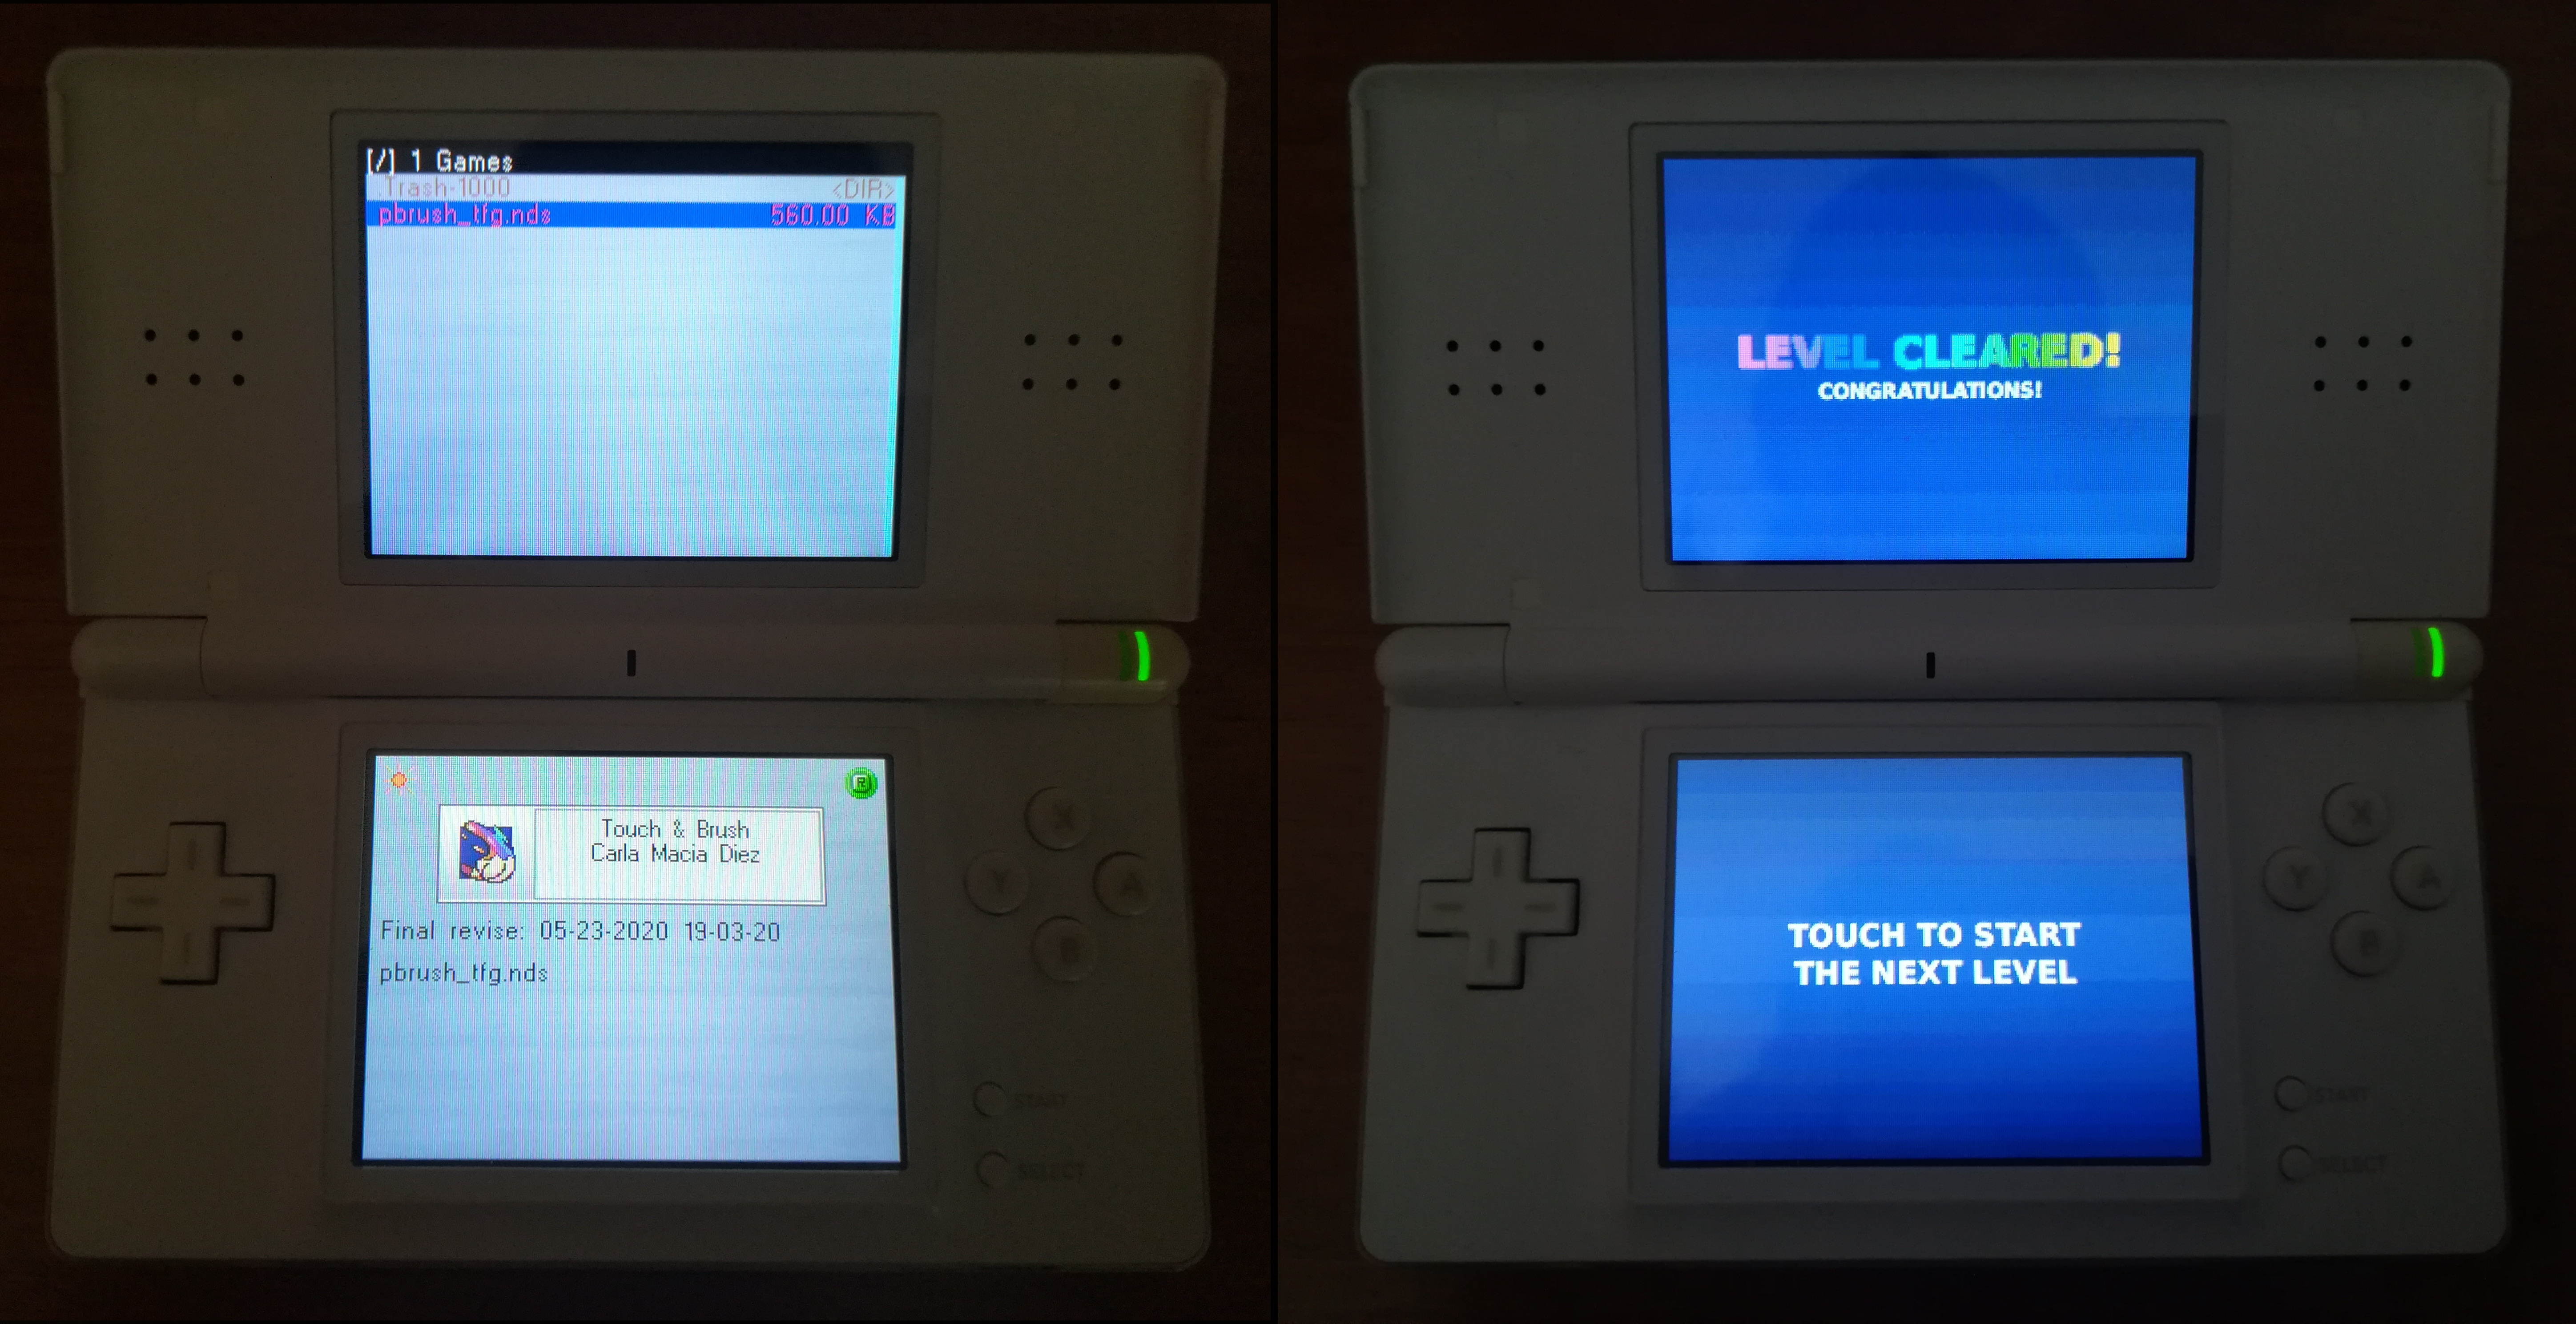
\includegraphics[width=0.8\textwidth]{archivos/final2.jpg}
  \caption{Pantalla de victoria y previsualización en la R4 de Touch \& Brush}
  \label{fig:final2}
\end{figure}

\vspace{0.5cm}

No obstante, para este proyecto existen diversas mejoras y ampliaciones las cuales pueden hacer que Touch \& Brush se convierta en un juego que los usuarios disfruten más. Dichas mejoras se centran \textbf{principalmente en adición de contenido}, ya que como hemos comentado, el juego actualmente se encuentra acabado. Estas se mencionan en el siguiente apartado.

\vspace{1cm}

\section{Mejoras}

Como hemos comentado, Touch \& Brush aún puede \textbf{mejorar} bastante más, si bien añadiendo \textbf{características que no se han podido implementar} o incluyendo \textbf{nuevas} ideas que han surgido durante el desarrollo. A continuación se detallan todas ellas.

 \vspace{0.5cm}

\begin{itemize}
\item \textbf{Incluir los enemigos y funcionalidades diseñadas que no se han podido implementar:} La principal mejora que se le podría aplicar al juego es la de incluir algunos aspectos que se diseñaron pero que no se han podido implementar. Por ejemplo, entre ellos están el sistema de \textbf{puntuación} en los niveles, el nivel de \textbf{jefe final} y el \textbf{aliado} que te permite recuperar vida durante la partida. Sin duda alguna, estas mejoras tendrían mucha prioridad, pues aportarían al juego mucha más diversión y dinamismo.

 \item \textbf{Mejora de pantallas:} Se podrían añadir las pantallas que fueron diseñadas, principalmente la pantalla de fin de partida y la de victoria. A pesar de que la de victoria está implementada en el juego, no es exáctamente igual a cómo se diseñó debido a un desajuste en la planificación, pues faltaría dotarle de más opciones (volver al menú y continuar), así como la visualización de la puntuación.

 \item \textbf{Añadir más niveles:} Otra mejora sería la de incorporar más niveles al juego, con enemigos que posean patrones más complejos, para así aumentar el contenido y la duración del juego.
 
  \item \textbf{Música:} La incorporación de una banda sonora es algo que puede aportar mucho al resultado final de un juego, ya sea por las canciones principales, las cuales ayudan al jugador a manifestar emociones de tensión, felicidad, miedo, ... o por los efectos de sonido, que ayudan a informarle al usuario de qué está ocurriendo en el juego.
 
 \item \textbf{Mejorar las animaciones:} A pesar de que la parte gráfica no era algo de gran peso en este proyecto, hay que considerar que para futuras revisiones podrían mejorarse las animaciones existentes y añadir algunas más (por ejemplo, el ataque de los enemigos). Esto es importante ya que mejoraría la calidad del producto final y aportaría más información al usuario sobre lo que pasa durante la partida. Además, también se podrían añadir incluso \textbf{cinemáticas} que cuenten la historia de cómo la protagonista ha llegado a esa situación.
 
 \item \textbf{Inluir un sistema de ayuda:} Una posible mejora para el juego, que beneficiaría la experiencia de usuario, sería la inclusión de un pequeño \textbf{tutorial} al principio del primer nivel que le enseñase al usuario que debe dibujar los patrones de los enemigos, tal y como hace Magic Cat Academy.
 
  \item \textbf{Menú de ajustes:} Para permitir al usuario ajustar algunas opciones como el idioma, volumen de la música y efectos de sonido, e incluso dificultad. Esta idea surgió durante las últimas iteraciones, al dejar a amigos y familiares probar el juego casi acabado. Algunos de ellos, sobre todo aquellos que no estaban muy relacionados con los videojuegos, no entendían qué debían hacer y acababan perdiendo en el primer nivel. No obstante, una vez lo intentaban por segunda vez y comenzaban a probar cosas (generalmente a tocar la pantalla), rápidamente ya comenzaban a matar a los enemigos y a avanzar en el juego.
  
  \item \textbf{Realizar la producción física del juego:} A pesar de que Touch \& Brush es un juego acabado, la producción de un juego en un cartucho es algo costoso, y si bien no se ha realizado todavía, es algo que acabará ocurriendo. Es por ello que es preferible invertir ese esfuerzo en un producto que considere que está mejor acabado visualmente y posee más contenido.
\end{itemize}

\vspace{0.5cm}

\section{Lecciones aprendidas}

Enfrentarme a un proyecto como este ha sido una experiencia que me ha permitido \textbf{aprender muchísimo}, no solo de los aspectos que ya esperaba, sino de muchos otros más.

\vspace{0.5cm}

He podido aprender mucho sobre la NDS y su arquitectura, y tener que ajustarme a hacer un juego para una \textbf{máquina específica con limitaciones} ha hecho que en varias ocasiones haya tenido que tomar una serie de decisiones, que más tarde y al haber obtenido más conocimiento según proseguía el desarrollo, he podido evaluar.

\vspace{0.5cm}

También, como en cualquier otro proyecto de ingeniería, he aprendido a \textbf{dar solución a una serie de problemas} usando lo que previamente he investigado. Si bien para desarrollos de proyectos que usan librerías o \textit{frameworks} más nuevos y con más soporte hay gran cantidad de ayuda e información en internet, para el caso de desarrollar para NDS es poco común ver eso. La gran mayoría de foros y librerías se encuentran desactualizados desde hace bastantes años, incluso la propia documentación de libnds me ha resultado excasa en muchas ocasiones. Esto ha hecho que a la hora de querer buscar más información acerca de, por ejemplo, una función, haya tenido que \textbf{ir también al propio código de la librería} y entender qué pretende hacer cada línea de código.

\vspace{0.5cm}

Por otro lado, este proyecto me ha permitido aprender sobre los \textbf{algoritmos de reconocimiento de gestos y escritura manuscrita}, así como las bases matemáicas que los sostentan. Solía ver este tipo de software una especie de caja negra y no pensaba que podía ser capaz de desarrollar el mío propio y funcionase correctamente. Si bien esto ha sido algo que no esperaba al principio cuando planteé hacer un juego para NDS, estoy bastante contenta de haber podido aprender de ello.

\vspace{0.5cm}

Además, también he aprendido sobre la importancia de un \textbf{buen diseño del juego inicial}, pues durante la fase de desarrollo el hecho de tener todos los aspectos del juego detallados (pantallas, mecánicas, comportamiento de los enemigos), me ha facilitado su implementación.

\vspace{0.5cm}

Por último, otro aspecto de mucha importancia durante este proyecto ha sido la \textbf{planificación}. Enfrentarse a un proyecto como este en solitario ha sido algo duro, y han surgido contratiempos en muchas ocasiones. Sin embargo, gracias a una buena planificación y dotar a las tareas de un orden de prioridad de modo que se podría conseguir un producto lo antes posible es lo que ha permitido que el proyecto haya tenido un buen resultado.

\vspace{0.5cm}

\section{Conclusión personal}

Personalmente, al haber podido llevar a cabo este proyecto me siento \textbf{muy satisfecha}, pues como ya he comentado, hacer un juego para NDS o crear un algoritmo de reconocimiento de escritura eran algo que hace un año me preguntaba cómo se hacían y veía fuera de mi alcance. Esto además, también me aporta la \textbf{confianza} necesaria para enfrentarme a \textbf{proyectos futuros} sin miedo a su complejidad.

\vspace{0.5cm}

Este ha sido un proyecto largo y en muchos momentos duro de afrontar. Especialmente porque ha habido momentos en los que mi motivación se ha visto muy reducida, ya sea por problemas personales, familiares o incluso la situación de la pandemia global provocada por el SARS-CoV-2. En cuanto a éste último, me gustaría señalar y agradecer la dedicación y esfuerzo de los profesores de la Universidad de Alicante, y en especial a mi tutor, Francisco Gallego, por su disponibilidad y ayuda a pesar de toda la situación.

\vspace{0.5cm}

No cabe duda de que seguiré mostrando a las personas Touch \& Brush para que puedan probarlo y obtener así nuevas opiniones e ideas para mejorarlo, haciendo que se convierta en un juego digno de competir con algunos títulos para la misma consola. El resultado de este proyecto me ha dejado tan contenta que mis ganas e ilusión de seguir trabajando en él en un futuro son casi las mismas que tuve al comenzarlo.

\vspace{0.5cm}

Como ya he comentado anteriormente, la NDS es una consola a la que siempre le he tenido mucho cariño, llegando a ser mi consola portátil preferida. He invertido mucho tiempo de mi infancia jugando a muchos de sus grandes títulos, y sin duda alguna haber conseguido hacer un juego completo para una cosa tan especial me hace inmensamente feliz.
